% Created 2016-08-17 Wed 14:38
\documentclass[tikz]{standalone}

\usepackage[utf8]{inputenc}
\usepackage[T1]{fontenc}
\usepackage{helvet}
\usepackage{../../templates/msc}

\renewcommand{\familydefault}{\sfdefault}

\tikzset{
every picture/.style={
line width=1pt
}}

\usepackage{tikz}
\author{Holger Karl}
\date{\today}
\title{}

\usetikzlibrary{backgrounds,fit,matrix,shapes.callouts}
\usepackage{forest}
\usepackage{tikzpeople}

\tikzset{spiral/.pic={  \draw [ very   thick,
  red!75,
  decorate,
  decoration={random steps,segment length=0.8pt,amplitude=0.1pt}, domain=0:6.5,variable=\t,smooth,samples=40]
  plot ({\t r}: {1+ 0.05*\t});}}


\begin{document}

  \begin{forest}
    for tree={ font=\ttfamily, grow'=0, child anchor=west, parent
      anchor=south, anchor=west, calign=first, edge path={
        \noexpand\path [draw, \forestoption{edge}] (!u.south west)
        +(7.5pt,0) |- node[fill,inner sep=1.25pt] {} (.child
        anchor)\forestoption{edge label}; }, before typesetting
      nodes={ if n=1 {insert before={[,phantom]}} {} }, fit=band,
      before computing xy={l=15pt}, } [<root>,name=root
    [.int,name=int] [.gov] [.mil] [.net] [.com [.google] [.apple] ]
    [.org [.ieee] [.acm] ] [.edu [.yale [.cs] [.chemistry] ]
    [.stanford] ] [.de,name=de [.paderborn] [.uni-paderborn,name=pb
    [.eim,name=eim] ] ] ]
    \begin{scope}[on background layer]
      % \draw [fill=green!10] (int.north west) rectangle (pb.east |-
      % de.north);
      % \draw [fill=blue!10] (de.north west) rectangle (pb.east |-
      % eim.south);
      \node [fill=green!10, fit= {(int.north west) (pb.east)
        (de.north)}] (g) {}; \node [fill=blue!10, fit= {(de.north
        west) (pb.east) (eim.south)}] (s) {}; \node [anchor=north
      east] at (g.north east) {Generic}; \node [anchor=north east] at
      (s.north east) {Specific};
    \end{scope}
  \end{forest}

%--------------------


\begin{comment}
  \begin{forest}
    for tree={ font=\ttfamily, grow'=0, child anchor=west, parent
      anchor=south, anchor=west, calign=first, edge path={
        \noexpand\path [draw, \forestoption{edge}] (!u.south west)
        +(7.5pt,0) |- node[fill,inner sep=1.25pt] {} (.child
        anchor)\forestoption{edge label}; }, before typesetting
      nodes={ if n=1 {insert before={[,phantom]}} {} }, fit=band,
      before computing xy={l=15pt}, } [<root>,name=root
    [.int,name=int] [.gov] [.mil] [.net] [.com [.google] [.apple] ]
    [.org [.ieee] [.acm] ] [.edu [.yale [.cs]
    [.chemistry,name=chemistry] ] [.stanford] ] [.de,name=de
    [.paderborn] [.uni-paderborn,name=pb [.eim,name=eim] ] ] ]
    \node[database] (rs) at (root -| 5,0) {}; \node[database] (rd) at
    (de -| 5,0) {}; \node[database] (rp) at (pb -| 5,0) {};
    \node[database] (reim) at (eim -| 5,0) {}; \node[alice] (client)
    at (chemistry -| 5,0) {C};
  % 
    \draw [->] (client.60) -- (client.60 -| 6,0) |- (rs.330); \draw
    [->] (rs) -| (client.20 -| 6.5,0) -- (client.20);
  %
    \draw [->] (client.280) -- (client.280 -| 6,0) |- (rd.30); \draw
    [->] (rd) -| (client.290 -| 6.5,0) -- (client.290);
  %
    \draw [->] (client.300) -- (client.300 -| 6,0) |- (rp.30); \draw
    [->] (rp) -| (client.3100 -| 6.5,0) -- (client.310);
  \end{forest}
\end{comment}


\begin{tikzpicture}
  \node  (cl) {Client resolver}; 
  \node [alice,above=0cm of cl] {}; 

  \node [database, right=of cl] (root)  {Root }; 
  \node [database, right=of root] (dnsde)  {de }; 
  \node [database, right=of dnsde] (dnspb)  {upb }; 
  \node [database, right=of dnspb] (dnseim)  {eim }; 

  % \draw[->] (cl.350) to [out=350,in=240]  (root.240); 
  % \draw[->] (root.270) to [out=270,in=240]   (cl.330) ; 

  \draw [->] (cl.350) -- ([yshift=-0.5cm]cl.350)  -| node [near start,
  auto] {(1)} (root.240); 
  \draw [->] (root.300) |- node[auto, near end] {(2)}
  ([yshift=-0.6cm]cl.340)  -- (cl.340); 
   
  \draw [->] (cl.330) -- ([yshift=-1.5cm]cl.330)  -| node [near start,
  auto] {(3)} (dnsde.240); 
  \draw [->] (dnsde.300) |- node[auto, near end] {(4)}
  ([yshift=-1.7cm]cl.320)  -- (cl.320); 

  \draw [->] (cl.300) -- ([yshift=-2.5cm]cl.300)  -| node [near start,
  auto] {(5)} (dnspb.240); 
  \draw [->] (dnspb.300) |- node[auto, near end] {(6)}
  ([yshift=-2.7cm]cl.280)  -- (cl.280); 

  \draw [->] (cl.250) -- ([yshift=-3.5cm]cl.250)  -| node [near start,
  auto] {(7)} (dnseim.240); 
  \draw [->] (dnseim.300) |- node[auto, near end] {(8)}
  ([yshift=-3.7cm]cl.230)  -- (cl.230); 

\end{tikzpicture}


%recursive resolution 

\begin{tikzpicture}
  \node  (cl) {Client resolver}; 
  \node [alice,above=0cm of cl] {}; 

  \node [database, right=of cl] (root)  {Root }; 
  \node [database, right=of root] (dnsde)  {de }; 
  \node [database, right=of dnsde] (dnspb)  {upb }; 
  \node [database, right=of dnspb] (dnseim)  {eim }; 

  % \draw[->] (cl.350) to [out=350,in=240]  (root.240); 
  % \draw[->] (root.270) to [out=270,in=240]   (cl.330) ; 

  \draw [->] (cl.300) -- ([yshift=-1cm]cl.300)  -| node [near start,
  auto] {(1)} (root.210); 

  \draw [->] (root.330) |- node[auto, near end] {(2)}
  ([yshift=-1cm]dnsde.210)  -- (dnsde.210); 
   
  \draw [->] (dnsde.330) |- node[auto, near end] {(3)}
  ([yshift=-1cm]dnspb.210)  -- (dnspb.210); 

  \draw [->] (dnspb.330) |- node[auto, near end] {(4)}
  ([yshift=-1cm]dnseim.210)  -- (dnseim.210); 

  \draw [->] (dnseim.240) --  
  ([yshift=-1.5cm]dnseim.240)  -|  node[auto, near start] {(5)} (dnspb.300); 

  \draw [->] (dnspb.240) --  
  ([yshift=-1.5cm]dnspb.240)  -|  node[auto, near start] {(6)} (dnsde.300); 


  \draw [->] (dnsde.240) --  
  ([yshift=-1.5cm]dnsde.240)  -|  node[auto, near start] {(7)} (root.300); 

  \draw [->] (root.240) --  
  ([yshift=-1.5cm]root.240)  -|  node[auto, near start] {(8)} (cl.240); 

\end{tikzpicture}

%------------------ DNS TABLE 


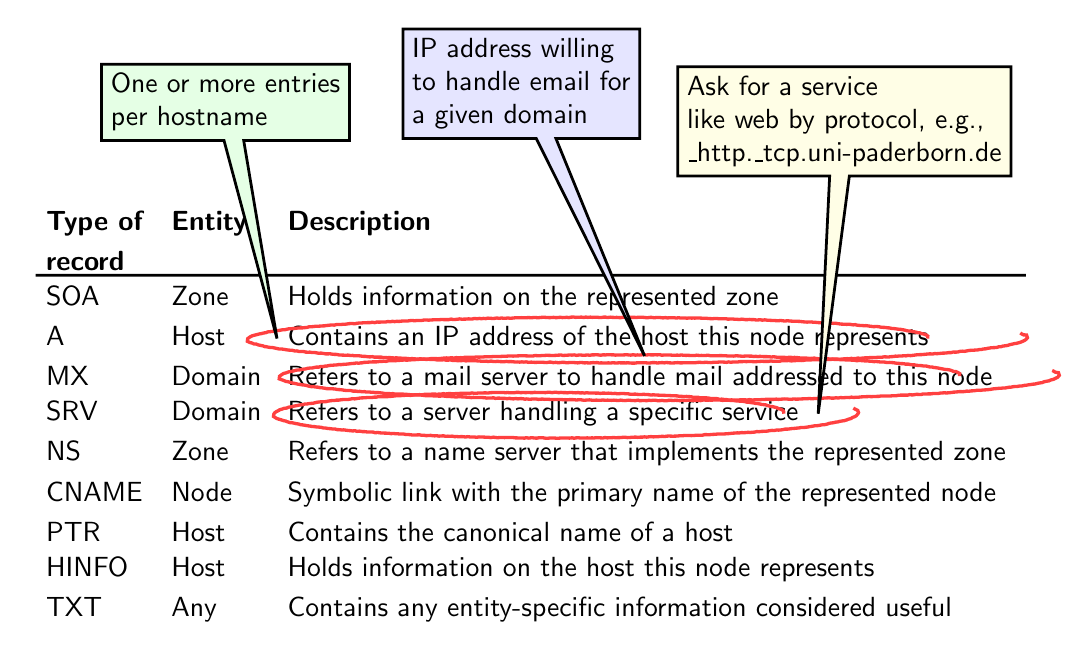
\begin{tikzpicture}[align=center]
\matrix (m) [matrix of nodes,
    column sep=-\pgflinewidth, 
    row sep=-\pgflinewidth,
    % nodes={rectangle, draw},
    column 1/.style={anchor=base west}, 
    column 2/.style={anchor=base west}, 
    column 3/.style={anchor=base west}, 
    ]{
      % 
    \textbf{Type of}   & \textbf{Entity}  & \textbf{Description} \\
    \textbf{record} & & \\
    SOA & Zone  & 
    Holds information on the represented
    zone 
    \\ 
    A & Host & |(a)| Contains an IP address of the host this node represents
    \\ 
    MX & Domain & 
     |(mx)| Refers to a mail server to handle mail addressed to this node
    \\
    SRV & Domain & 
     |(srv)| Refers to a server handling a specific service
    \\
    NS & Zone &
    Refers to a name server that implements the represented zone
    \\
    CNAME & Node & 
    Symbolic link with the primary name of the represented node
    \\
    PTR & Host & 
    Contains the canonical name of a host
    \\
    HINFO & Host & 
    Holds information on the host this node represents
    \\
    TXT & Any & 
    Contains any entity-specific information considered useful 
    \\
  };  
   \draw (m-3-1.north west) -- (m-3-3.north east -| m-7-3.east);
   % red circles: 
   \path  (a) pic [xscale=4, yscale=0.25] {spiral}; 
   \path  (mx) pic [xscale=4, yscale=0.25] {spiral}; 
   \path  (srv) pic [xscale=3, yscale=0.25] {spiral}; 
   % 
   % callouts: 
   \node [anchor=west, align=left,rectangle callout, fill=green!10, draw, callout absolute
   pointer={(a.west)}] at ([xshift=0cm,yshift=3cm]a.east -| m-1-1.north) {One or more
   entries\\per hostname};
 % 
   \node [anchor=south, align=left,rectangle callout, fill=blue!10, draw, callout absolute
   pointer={(mx.north)}] at ([xshift=2cm,yshift=3cm]mx.east -| m-1-3.north) {IP
     address willing \\to handle  email for\\ a given domain};
   % 
   \node [anchor=south, align=left,rectangle callout, fill=yellow!10, draw, callout absolute
   pointer={(srv.east)}] at ([xshift=5cm,yshift=3cm]srv.east -| m-1-3.east) {Ask
     for a service \\ like web by protocol, e.g.,  \\
     \_http.\_tcp.uni-paderborn.de};
\end{tikzpicture} 


%-----------------

  \begin{forest}
    for tree={ font=\ttfamily, grow'=0, child anchor=west, parent
      anchor=south, anchor=west, calign=first, edge path={
        \noexpand\path [draw, \forestoption{edge}] (!u.south west)
        +(7.5pt,0) |- node[fill,inner sep=1.25pt] {} (.child
        anchor)\forestoption{edge label}; }, before typesetting
      nodes={ if n=1 {insert before={[,phantom]}} {} }, fit=band,
      before computing xy={l=15pt}, } [<root>,name=root
    [.int,name=int] [.com [.google] [.apple] ]
    [.edu, draw, rounded corners, fill=blue!10,
      [.yale, name=yale 
        [.chemistry, name=yalechem ] 
        [.cs, name=yalecs 
          [.ai, name=yaleai ]
          [.robotics, name=yalerob]
        ] 
    ]
    [.stanford] ] 
    % [.de,name=de, draw, circle
    %   [.paderborn,name=pb] 
    %   [.uni-paderborn,name=upb
    %   [.eim,name=eim] ] 
    %   ] 
    ]
    % background 
    \begin{scope}[on background layer]
    %   % \draw [fill=green!10] (int.north west) rectangle (pb.east |-
    %   % de.north);
    %   % \draw [fill=blue!10] (de.north west) rectangle (pb.east |-
    %   % eim.south);
    %   \node [fill=green!10, fit= {(int.north west) (upb.east)
    %     (de.north)}] (g) {}; 
    %   \node [fill=blue!10, fit= {(de.north
    %     west) (upb.east) (eim.south)}] (s) {}; 
    %   \node [anchor=north east] at (g.north east) {Generic}; 
    %   \node [anchor=north east] at  (s.north east) {Specific};
    % DNS servers 
      \node [draw, rounded corners, fit=(yale) (yalechem) ,
      inner sep =0, fill=green!10] {}; 
      \node [draw, rounded corners, fit=(yalecs) (yaleai) (yalerob),
      inner sep =0, fill=yellow!10] {}; 
    \end{scope}
  \end{forest}


\end{document}